\chapter{Proxy模式}
\section{代理模式的概念}
\subsection{定义}
代理模式的定义:由于某些原因需要给某对象提供一个代理以控制对该对象的访问。这时,访问对象不适合或者不能直接引用目标对象,代理对象作为访问对象和目标对象之间的中介。
\subsection{优点}
\begin{enumerate}
	\item 代理模式在客户端与目标对象之间起到一个中介作用和保护目标对象的作用;
	\item 代理对象可以扩展目标对象的功能;
	\item 代理模式能将客户端与目标对象分离,在一定程度上降低了系统的耦合度;
\end{enumerate}
\subsection{缺点}
\begin{enumerate}
	\item 在客户端和目标对象之间增加一个代理对象,会造成请求处理速度变慢;
	\item 增加了系统的复杂度。
\end{enumerate}
\subsection{代理模式的角色}
\begin{enumerate}
	\item Subject主体:通过接口或抽象类声明真实主题和代理对象实现的业务方法。
	\item Proxy代理人:提供了与真实主题相同的接口,其内部含有对真实主题的引用,它可以访问、控制或扩展真实主题的功能。
	\item RealSubject实际的主体:实现了抽象主题中的具体业务,是代理对象所代表的真实对象,是最终要引用的对象。
	\item Client请求者:使用Proxy模式,但并不包含在代理模式中。
\end{enumerate}
\subsection{应用场景}
\begin{enumerate}
	\item 远程代理,这种方式通常是为了隐藏目标对象存在于不同地址空间的事实,方便客户端访问。
	\item 虚拟代理,这种方式通常用于要创建的目标对象开销很大时。例如,下载一幅很大的图像需要很长时间,因某种计算比较复杂而短时间无法完成,这时可以先用小比例的虚拟代理替换真实的对象,消除用户对服务器慢的感觉。
	\item 安全代理,这种方式通常用于控制不同种类客户对真实对象的访问权限。
	\item 智能指引,主要用于调用目标对象时,代理附加一些额外的处理功能。例如,增加计算真实对象的引用次数的功能,这样当该对象没有被引用时,就可以自动释放它。
	\item 延迟加载,指为了提高系统的性能,延迟对目标的加载。例如,Hibernate 中就存在属性的延迟加载和关联表的延时加载。
\end{enumerate}
\section{代理模式实现——例一}
注:
\par Printer并不知道PrinterProxy的存在,只有真正使用print时,才生成实例。
\begin{figure}[!h]
	\centering
	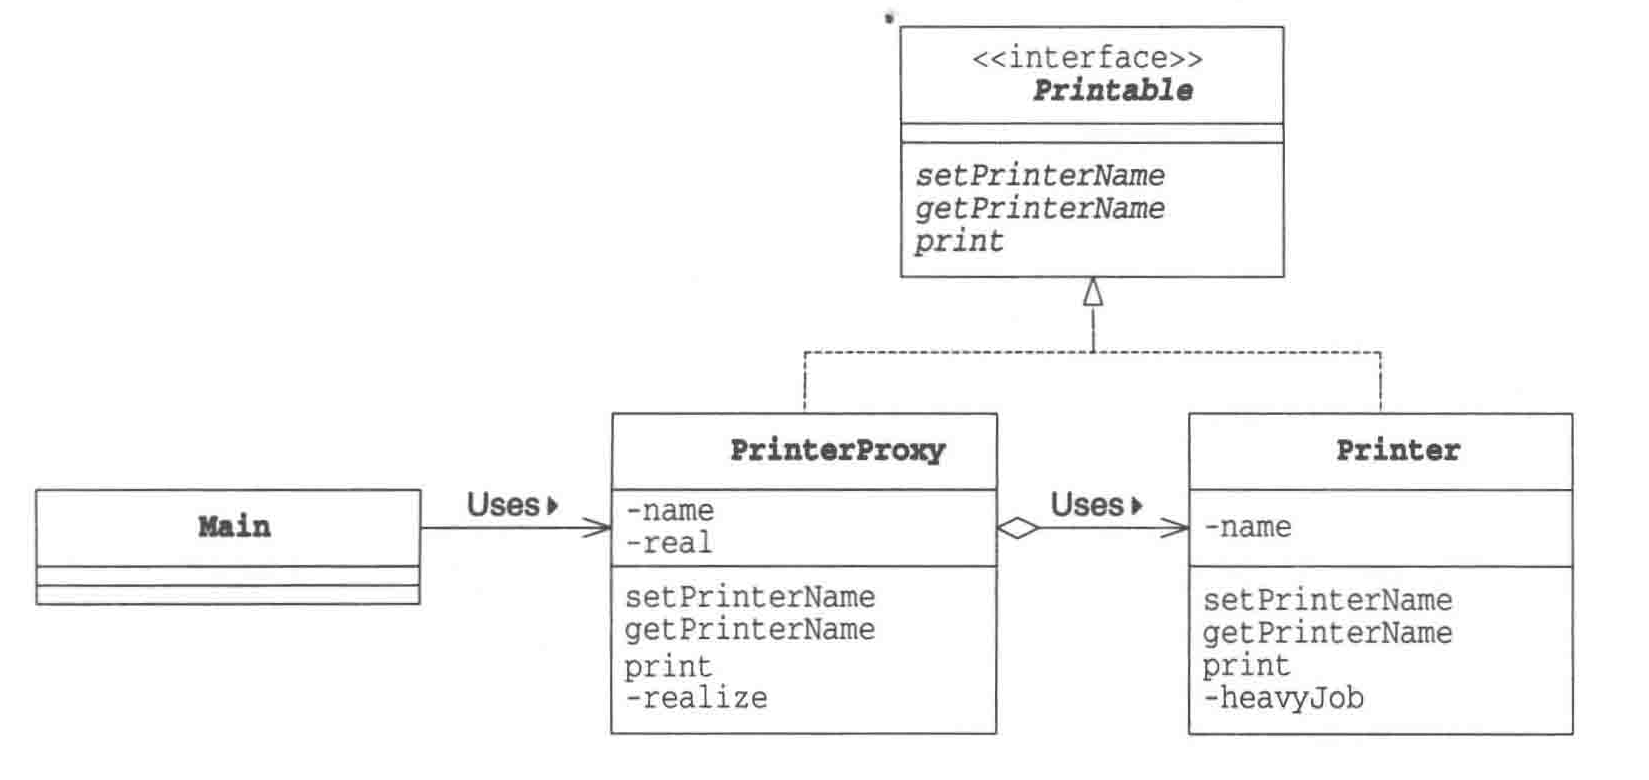
\includegraphics[width=0.8\textwidth]{image/21-1}
	\caption{代理模式的类图}
\end{figure}
\begin{figure}[!h]
	\centering
	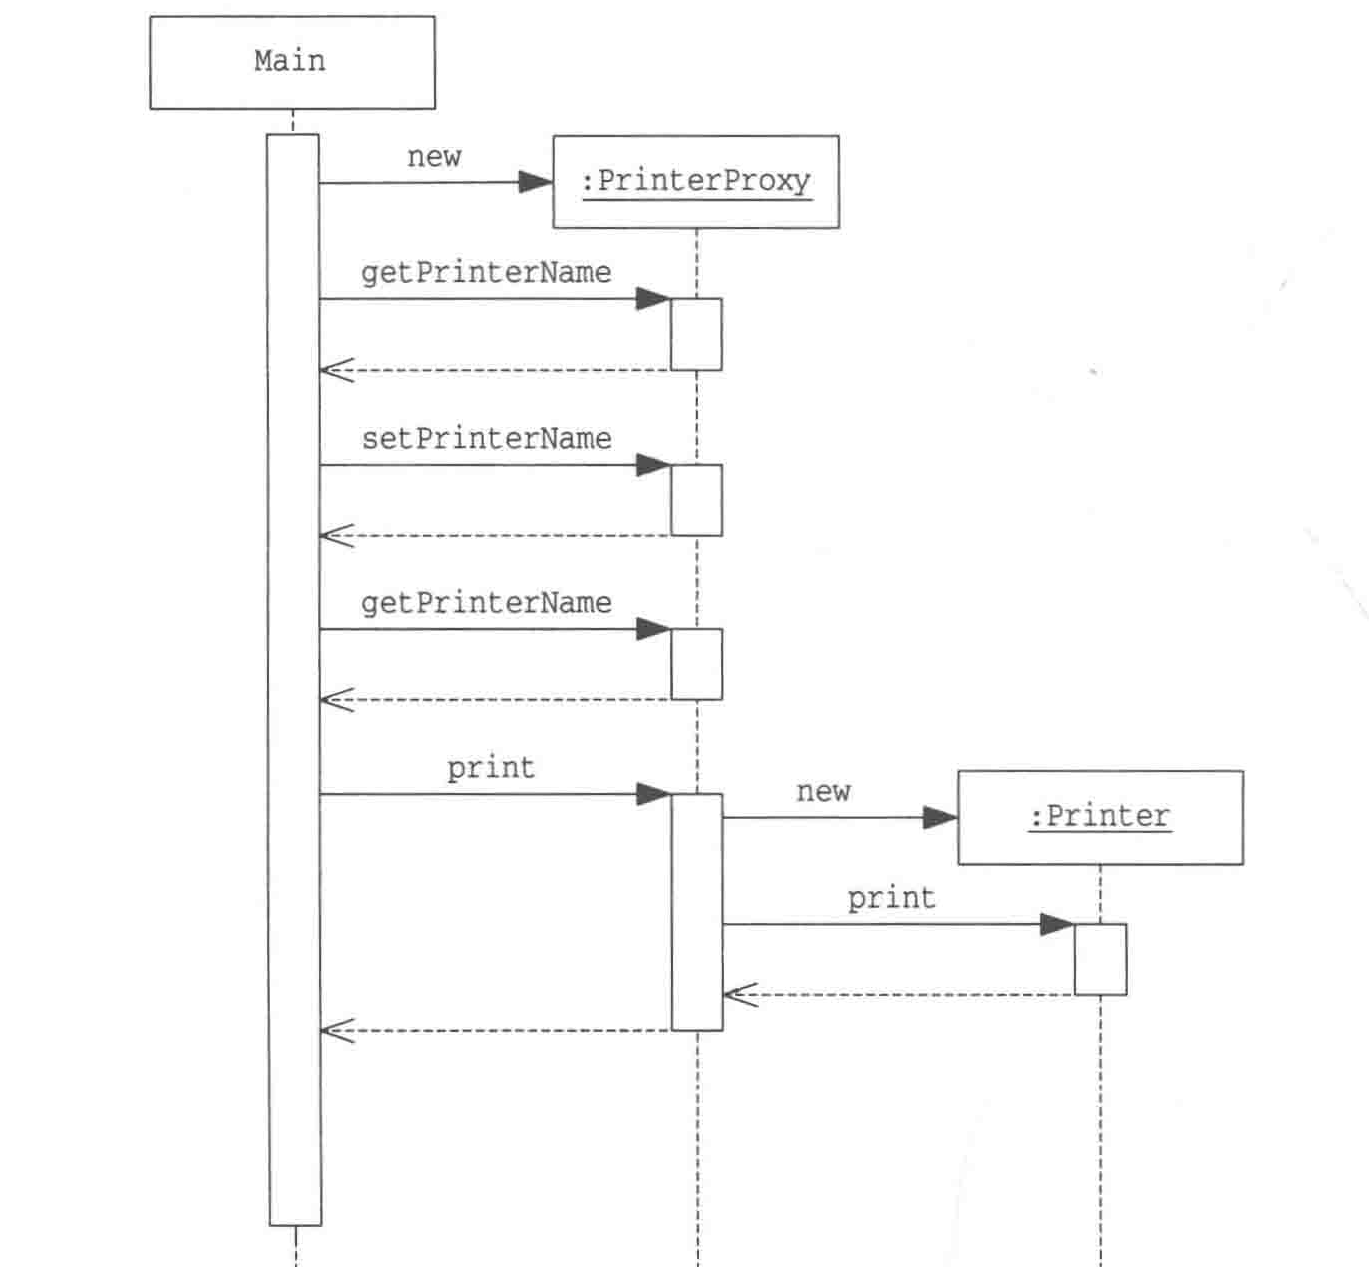
\includegraphics[width=0.8\textwidth]{image/21-2}
	\caption{代理模式的顺序图}
\end{figure}
\begin{lstlisting}
public interface Printable {
	public abstract void setPrinterName(String name);   // 设置名字
	public abstract String getPrinterName();            // 获取名字
	public abstract void print(String string);          // 显示文字(打印输出)
}
\end{lstlisting}
\begin{lstlisting}
public class Printer implements Printable {
	private String name;
	public Printer() {
		heavyJob("正在生成Printer的实例");
	}
	public Printer(String name) {                   // 构造函数
		this.name = name;
		heavyJob("正在生成Printer的实例(" + name + ")");
	}
	public void setPrinterName(String name) {       // 设置名字
		this.name = name;
	}
	public String getPrinterName() {                // 获取名字
		return name;
	}
	public void print(String string) {              // 显示带打印机名字的文字
		System.out.println("=== " + name + " ===");
		System.out.println(string);
	}
	private void heavyJob(String msg) {             // 重活
		System.out.print(msg);
		for (int i = 0; i < 5; i++) {
			try {
				Thread.sleep(1000);
			} catch (InterruptedException e) {
			}
			System.out.print(".");
		}
		System.out.println("结束。");
	}
}
\end{lstlisting}
\begin{lstlisting}
public class PrinterProxy implements Printable {
	private String name;            // 名字
	private Printer real;           // “本人”
	public PrinterProxy() {}
	public PrinterProxy(String name) {      // 构造函数
		this.name = name;
	}
	public synchronized void setPrinterName(String name) {  // 设置名字
		if (real != null) {
			real.setPrinterName(name);  // 同时设置“本人”的名字
		}
		this.name = name;
	}
	public String getPrinterName() {    // 获取名字
		return name;
	}
	public void print(String string) {  // 显示
		realize();
		real.print(string);
	}
	private synchronized void realize() {   // 生成“本人”
		if (real == null) {
			real = new Printer(name);
		}
	}
}
\end{lstlisting}
\begin{lstlisting}
public class Main {
	public static void main(String[] args) {
		Printable p = new PrinterProxy("Alice");
		System.out.println("现在的名字是" + p.getPrinterName() + "。");
		p.setPrinterName("Bob");
		System.out.println("现在的名字是" + p.getPrinterName() + "。");
		p.print("Hello, world.");
	}
}
\end{lstlisting}
\begin{lstlisting}
//output
现在的名字是Alice。
现在的名字是Bob。
正在生成Printer的实例(Bob).....结束。
=== Bob ===
Hello, world.
\end{lstlisting}
\section{代理模式实现——例二}
\begin{figure}[!h]
	\centering
	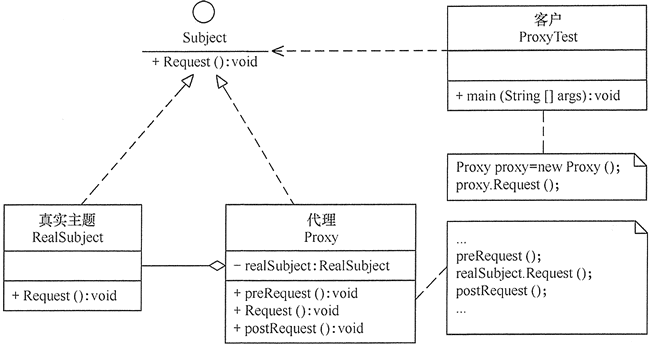
\includegraphics[width=0.8\textwidth]{image/21-3}
	\caption{代理模式的结构图}
\end{figure}
\begin{lstlisting}
//抽象主题
interface Subject {
	void Request();
}

//真实主题
class RealSubject implements Subject {
	public void Request() {
		System.out.println("访问真实主题方法...");
	}
}
\end{lstlisting}
\begin{lstlisting}
//代理
class Proxy implements Subject {
	private RealSubject realSubject;
	
	public void Request() {
		if (realSubject == null) {
			realSubject = new RealSubject();
		}
		preRequest();
		realSubject.Request();
		postRequest();
	}
	
	public void preRequest() {
		System.out.println("访问真实主题之前的预处理。");
	}
	
	public void postRequest() {
		System.out.println("访问真实主题之后的后续处理。");
	}
}
\end{lstlisting}
\begin{lstlisting}
public class ProxyTest {
	public static void main(String[] args) {
		Proxy proxy = new Proxy();
		proxy.Request();
	}
}
\end{lstlisting}
\begin{lstlisting}
//output
访问真实主题之前的预处理。
访问真实主题方法...
访问真实主题之后的后续处理。
\end{lstlisting}
\section{模式扩展}
代理模式中,代理类中包含了对真实主题的引用,这种方式存在两个缺点:
\begin{enumerate}
	\item 真实主题与代理主题一一对应,增加真实主题也要增加代理;
	\item 设计代理以前真实主题必须事先存在,不太灵活。采用动态代理模式可以解决以上问题,如 SpringAOP。
\end{enumerate}
\begin{figure}[!h]
	\centering
	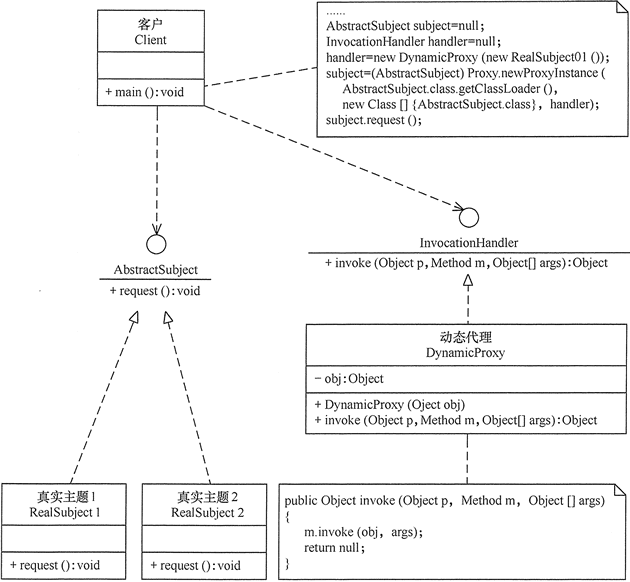
\includegraphics[width=0.8\textwidth]{image/21-4}
	\caption{动态代理模式的结构图}
\end{figure}
\section{思路扩展}
\begin{enumerate}
	\item 使用代理人来提升速度;
	\item 划分代理人和本人,可以使它们成为独立的组件,在进行修改时不会互相产生影响;
	\item 代理与委托:代理人只代理它能解决的问题,当不能完成时,会转交给本人处理。
	\item 透明性:继承与相同接口,具有透明性。
	\item HTTP代理:位于HTTP服务器和HTTP客户端之间,为Web页面提供高速缓存的功能的软件。
\end{enumerate}
\section{各种Proxy模式}
\begin{enumerate}
	\item Virtual Proxy虚拟代理:只有真正需要实例时,才生成和初始化实例;
	\item Remote Proxy远程代理:可以忽略RealSubject位置,透明地调用它。
	\item Access Proxy:访问限制。
\end{enumerate}
\section{相关设计模式}
\begin{enumerate}
	\item Adapter模式:Adapter适配了两种不同接口的对象,以使得它们可以一同工作,
	而Proxy角色与RealSubject角色接口是相同的。
	\item Decorator模式:Decorator模式目的在于增加新的功能,Proxy更注重设置代理人减轻本人的
	工作负担。
\end{enumerate}